\chapter{Visible light communication}

\section {Brief history of Visible Light Communication.}
The use of light to send messages is a very old idea. Fire and smoke signalling were used in ancient civilizations. For example, the ancient Greeks used polished shields to reflect sunlight to signal in the battle and Roman records indicate that polished metal plates were used as mirrors to reflect sunlight for long distance signalling. Chinese started using fire beacons followed by the Romans and American Indians using
smoke signals.

In the early 1800s, the US military used a wireless solar telegraph called “Heliograph” which is shown in figure that signals using
Morse code flashes of sunlight reflected by a mirror. The flashes are produced by momentarily pivoting the mirror, or by interrupting the beam with a shutter. The diagram of heliograph is shown in Figure \ref{helio}. The navy often uses blinking lights, i.e. Aldis lamps, to
send messages also using Morse code from one ship to another.
\begin{figure}[h]
\begin{center}
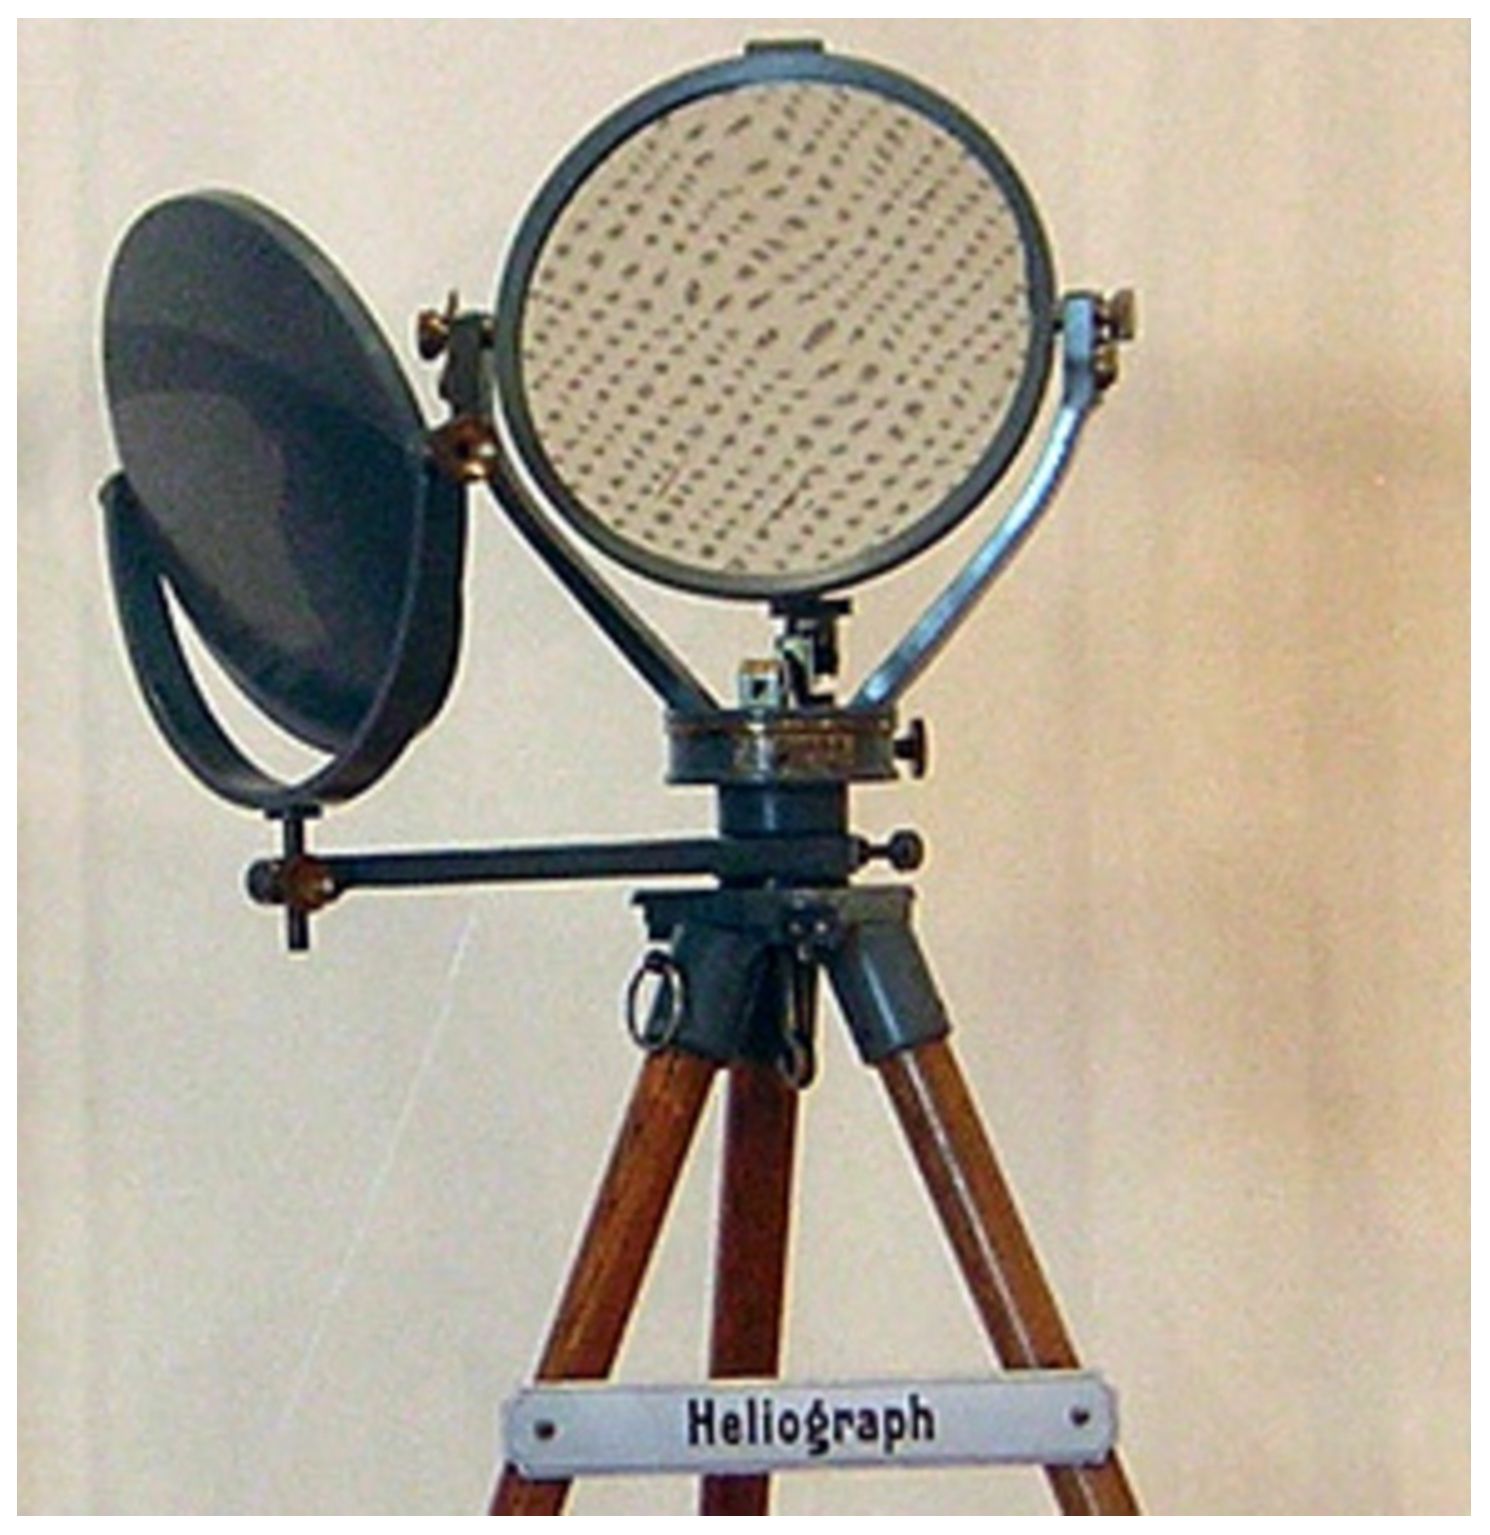
\includegraphics[width=3.0in]{heliograph.eps}
\caption{Heliograph \cite{r17}.} \label{helio}
\end{center}
\end{figure}

\pagebreak

In 1880, the first example of VLC technology was demonstrated by Alexander Graham Bell with his “photophone” that used sunlight
reflected off a vibrating mirror and a selenium photo cell to send voice on a light beam. The transmitter and receiver of photophone is shown in Figure \ref{sun}.
\begin{figure}[h]
\begin{center}
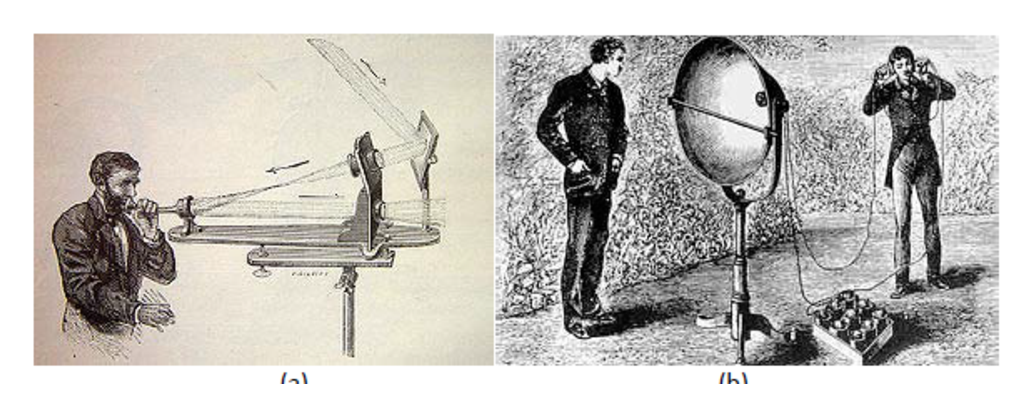
\includegraphics[width=4.0in]{sunlight.eps}
\caption{(a) Photophone transmitter. (b) Photophone receiver and handset.} \label{sun}
\end{center}
\end{figure}

Until the late 1960s, radio and radar communications were more successful than optical communications
(OC). OC started to get real attention with the invention of the light amplification by stimulated emission of
radiation (laser) and the laser diode (LD) in the 1960s, followed in the 1970s by the development of lowloss
optical fibres (OFs) as a medium for transmitting information using light, the invention of the OF amplifier in the 1980s, and the invention of the in-fibre Bragg grating in the 1990s. These inventions formed the basis for the telecommunications revolution of the late 20th century and provided the infrastructure for the Internet. The Nobel Prize in physics 2009 went to three scientists (Charles K. Kao, Willard S. Boyle,
George E. Smith) who have played important roles in shaping the modern information technology due to
their ground breaking achievements concerning the transmission of light in fibers for optical
communication. Advancements in basic opto-electronic devices, such as LEDs (light emitting diodes) and
LDs, p-intrinsic-n (PIN) photodiodes (PDs) and avalanche photo-diodes (APDs) and various optical
components have attracted engineers to consider optical sources for wireless data transmission which has
led to modern optical wireless communications (OWC).

The first indoor OWC system was developed over 25 years ago. In 1979, an indoor OWC system was
presented by Gfeller and Bapst. In their system, diffuse optical radiation in the near-IR region was
utilised to interconnect a cluster of terminals located in a room to a common cluster controller.
During the last ten years, we have witnessed the emergence of visible light communications (VLC) fuelled
by solid-state lighting (SSL) technology. SSL is a rapidly developing area, both in terms of commercial
exploitation, and academic and industrial research. LEDs with a wide range of colours are available,
including white light. The output power as well as device efficiencies are increasing rapidly. The field of
applications is also expanding. White LEDs are commonly used as replacements for incandescent lamps due
to more than 10 times improved energy efficiency. Therefore, LED lighting is set to revolutionise the way
we illuminate our homes, offices, public buildings and streets.

These SSL sources, being semiconductor devices, come with an additional feature. Their light intensity can
be varied at very high speeds, and so their functionality can be extended by means of intensity modulation
(IM) to also become a wireless communication device.

VLC originated in Japan and the visible light communications consortium (VLCC) was established in
November 2003. The VLCC has major companies in Japan on board and aims at publicising and
standardising VLC technology. The formation of the VLCC has stimulated worldwide interest in VLC
technology, and the first IEEE standard for VLC - IEEE 802.15.7 – has emerged recently. University of
Edinburgh academics have worked on VLC since 2004 and have developed enhanced modulation schemes
that enable high data rates to be achieved using standard LED light bulbs.

%%%%%%%%%%%%%%%%%%%%%%%%%%
%The idea of using light as a communication medium was implemented by Alexander
%Graham Bell in 1880 with his invention of the photophone, a device that transmitted a
%voice signal on a beam of light. Bell focused sunlight with a mirror and then talked into a
%mechanism that vibrated the mirror. The vibrating beam was picked up by the detector at
%the receiving end and decoded back into the voice signal, the same procedure as the
%phone did with electrical signals. But Bell could not generate a useful carrier frequency,
%nor was he able to transmit the light beam from point to point. Obstacles in nature such as
%fog and rain — which could interfere with the photophone — made Bell stop any future research into his invention [7]. With the invention of LED (Light Emitting Diode), the
%idea of using light as a communication medium has started again. VLC uses white Light
%Emitting Diodes (LED), which send data by flashing light at speeds undetectable to the
%human eye. One major advantage of VLC is that we can use the infrastructure around us
%without having to make any changes to it. LEDs’ ability to transfer information signals
%over light ( light which is between 400THz to 800THz of frequency and whose
%wavelength is between 400nm to 700nm ) makes it a very good communication medium.
%Now the light we use in our daily life can not only be used for providing light but also for
%communication.
%%%%%%%%%%%%%%%%%%%%%%%%%%

%Human being has used a visible light source as a form of data transmission since ancient
%times.Since ancient times humans are using it in simple form. For example, in old times to give war signals, they used reflection of sunlight using brushed iron piece or smoke in day time and at night they were using fire to give signals. That was the best and very effective way to inform others by giving signal like this for that time as technology was not developed enough.

%\begin{figure}[h]
%\begin{center}
%\includegraphics[width=4.0in]{history.eps}
%\caption{Historical perspective of Visible Light Communications.} \label{his}
%\end{center}
%\end{figure}
%
%\begin{itemize}
%  \item Sunlight
%  The heliograph was used to send information over large distances by using reflecting
%mirrors.
%In 1880, Alexander Graham Bell invented the “Photophone”, which allowed
%transmitting sounds over long distances on a beam of light. It is considered as the first
%sophisticated wireless communications device.

%\begin{figure}[h]
%\begin{center}
%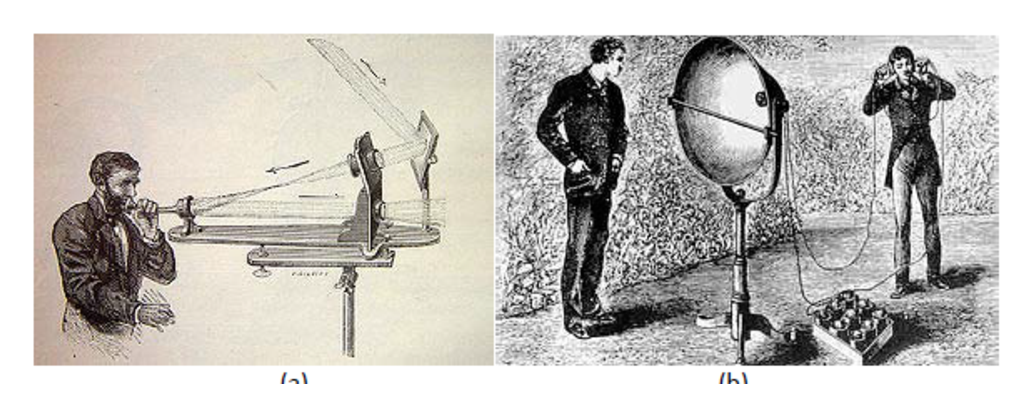
\includegraphics[width=4.0in]{sunlight.eps}
%\caption{(a) Photophone transmitter. (b) Photophone receiver and handset.} \label{sun}
%\end{center}
%\end{figure}
%\pagebreak
%
%  \item Fire
%
%  \item Lamps
%
%  \item LEDs

%\end{itemize}

\section {Spectrum Analysis}
Since Visible light communication is a data communication technology that uses visible light between 380 nm and 780 nm. These wavelengths correspond to a frequency range of approximately 384 THz to 789 THz. In Figure \ref{mux} and \ref{vlc}, we can see a diagram of the visible light spectrum. The visible light spectrum is 10000 times larger than that of radio spectrum.	

\begin{figure}[h]
\begin{center}
\includegraphics[width=4.0in]{spectrum.eps}
\caption{Visible light portion in electromagnetic spectrum \cite{r17}.} \label{mux}
\end{center}
\end{figure}

\begin{figure}[h]
\begin{center}
\includegraphics[width=4.0in]{vlcspectrum.eps}
\caption{visible light spectrum.} \label{vlc}
\end{center}
\end{figure}

\pagebreak

\section {Characteristics of VLC}

The main characteristics of this technology are summarized below \cite{r1}: 
\begin{itemize}
  \item Bandwidth :
The bandwidth is virtually not limited, it offers a frequency band of  approximately 400THz.
  \item Efficiency :
VLC is highly energy efficient since illumination and transmission of data are done at the same time.
  \item Data Rates :
VLC can achieve high data rates (hundreds of Mb/s) and it can therefore be used for high speed wireless communications.
  \item Cost :
As VLC uses the visible light spectrum it is free of cost. Furthermore, transmitters and receivers are cheap.
  \item Human Safety :
VLC is harmless to human health and it is not injurious to the human eye.
  \item Omnipresent Nature :
We have the infrastructure because there are already a lot of LED-based lights installed in the world which are potential VLC transmitters and therefore we can use them for communications.
  \item Security :
As light waves do not penetrate opaque objects they can not  be intercepted, so it offers a very secure communication. It is very difficult for an intruder to make use of your signal.
  \item Visibility :
It is great to see data being communicated by a beam of light. What you see is what you send!
 % \item 
\end{itemize}




%Traditiovnally, diggfital signal processing (DSP) algorithms are
%implemented using general-purpose (programmable) D
%in section \ref{organization},we haveeee further,subsection\ref{partt1}
%\begin{tabular}{|c|c|}
%                                                                         \hline
%                                                                         % after \\: \hline or \cline{col1-col2} \cline{col3-col4} ...
%                                                                         x & y \\
%                                                                         1 & 2 \\
%                                                                         \hline
%                                                                       \end{tabular}
